\begin{section}{IV-replacement (stateful) attack}
\label{sec:iv_replacement_stateful}

\begin{figure}[!ht]
	\centering
	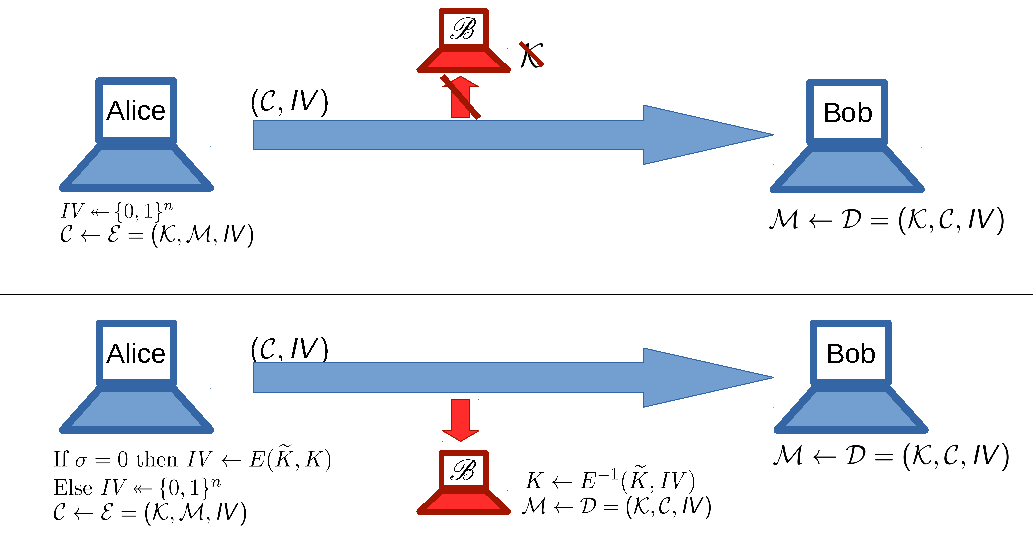
\includegraphics[width=\textwidth]{image/iv_replacement_stateful}
	\caption{IV replacement (stateful) attack.}
	\label{fig:iv_replacement_stateful}
\end{figure}

\begin{subsection}{Grundidee}

Der erste und simpelste Ansatz für eine ASA ist die IV replacement attack. Dieser Angriff zielt auf ein symmetrisches stateful Schema mit einem öffentlichen nonce ab. Ein solcher nonce könnte zum Beispiel ein Initialisierungsvektor sein. Grundidee ist es hierbei, dass der Schlüssel $\mathcal{K}$ im IV versteckt wird.

\end{subsection}

\begin{subsection}{Durchführung}

Zusammen mit dem Chiffretext $\mathcal{C}$ wird ein nonce übertragen, in diesem Beispiel der Initialisierungsvektor IV. Dieser ist Bestandteil der Verschlüsselung mit $\mathcal{E} = (\mathcal{K}, M, IV)$ und der Entschlüsselung mit $\mathcal{D} = (\mathcal{K}, C, IV)$. Im einfachsten Fall nehmen wir an, dass die $|IV|$ und die $|\mathcal{K}|$ identisch sind. Ausgenutzt wird hierbei der Pseudozufallsgenerator, der einen nicht verifizierbaren Zufall geniert. Der IV wird also als Geheimnisträger missbraucht. Der Status $\sigma$ dient hierbei auch als Status zur Erzeugung des IVs. Nur zu Beginn einer Verschlüsselung soll das Geheimnis $\mathcal{K}$ über den nonce verraten werden. Dieser Angriff kann eben so erweitert werden für $|\mathcal{K}| > |IV|$, indem immer nur Teile von $\mathcal{K}$ über den Status $\sigma$  hinweg verraten werden. Big Brother reproduziert sich den geheimen Schlüssel $\mathcal{K}$ mit der Umkehrfunktion $E^{-1}$ und seinem Masterschlüssel $\widetilde{\mathcal{K}}$.

\end{subsection}

\begin{subsection}{Entdeckbarkeit}

Eine solche Subversion ist unentdeckbar, wenn der vom Pseudo"-zufallszahlen"-generator (PRNG) erzeugte IV ununterscheidbar ist von einem zufällig gewähltem. Selbst für einen Beobachter der den Schlüssel $\mathcal{K}$ kennt ist so eine Subversion unentdeckbar. Allerdings steigt die Wahrscheinlich einer Entdeckung, wenn sich ein IV wiederholt. Dies wäre vorstellbar wenn das System resettet wird.

\end{subsection}

\end{section}